\documentclass[runningheads]{llncs}

\usepackage[utf8]{inputenc}
\usepackage[T1]{fontenc}
\usepackage{amsmath,amssymb}
\usepackage[dvipsnames]{xcolor}
\usepackage{mathtools}
\usepackage{mathpartir}        % inference rules (replaces curryst)
\usepackage{graphicx}
\usepackage{listings}
\usepackage{xcolor}
\usepackage{booktabs}
\usepackage{tikz}              % small Hasse diagram (replaces fletcher)
\usetikzlibrary{positioning}
\usepackage[hidelinks]{hyperref}

\graphicspath{{assets/}}
\DeclareGraphicsExtensions{.pdf,.png}

% ---------------------------------------------------------------------------
% Notation
% ---------------------------------------------------------------------------
\newcommand{\Chartreux}{\textsf{Chartreux}}
\newcommand{\lub}{\sqcup}
\newcommand{\squb}{\sqsubseteq}
\newcommand{\harpoon}{\rightharpoonup}
\newcommand{\coh}{\mathsf{Coh}}
\newcommand{\fhbsl}{\textsc{fhbsl}}
\newcommand{\Fin}{\mathrm{Fin}}
\newcommand{\Val}{\mathit{Val}}
\newcommand{\Var}{\mathit{Var}}
\newcommand{\Expr}{\mathit{Expr}}
\newcommand{\Stmt}{\mathit{Stmt}}
\newcommand{\Id}{\mathit{Id}}
\newcommand{\Cnt}{\mathit{Cnt}}
\newcommand{\AbsVal}{\mathit{AbsVal}}
\newcommand{\AbsConseq}{\mathit{AbsConseq}}
\newcommand{\AbsFact}{\mathit{AbsFact}}
\newcommand{\NodeKind}{\mathit{NodeKind}}
\newcommand{\NodeID}{\mathit{NodeID}}
\newcommand{\nonnull}{\mathit{nonnull}}
\newcommand{\knull}{\mathsf{null}}
\newcommand{\kInt}{\mathsf{Int}}
\newcommand{\kVar}{\mathsf{Var}}
\newcommand{\kisnull}{\mathsf{isnull}}
\newcommand{\kvar}{\mathsf{var}}
\newcommand{\kif}{\mathsf{if}}
\newcommand{\kelse}{\mathsf{else}}
\newcommand{\kwhile}{\mathsf{while}}
\newcommand{\kskip}{\mathsf{skip}}
\newcommand{\kassume}{\mathsf{assume}}
\newcommand{\kcall}{\mathsf{call}}
\newcommand{\kinvoke}{\mathsf{invoke}}
\newcommand{\kind}{\mathrm{kind}}
\newcommand{\aeval}{\mathrm{aeval}}
\newcommand{\exprConseq}{\mathrm{exprConseq}}
\newcommand{\admits}{\mathrm{admits}}
\newcommand{\fst}{\mathrm{fst}}
\newcommand{\snd}{\mathrm{snd}}
\newcommand{\dom}{\mathrm{dom}}
\newcommand{\pred}{\mathrm{pred}}
\newcommand{\succG}{\mathrm{succ}}
\newcommand{\some}{\mathrm{some}}
\newcommand{\summary}{\mathrm{summary}}
\newcommand{\FamilyChecked}{\mathsf{FamilyChecked}}
\newcommand{\Gk}{G_\kappa}
\newcommand{\sem}[1]{\ulcorner #1 \urcorner}
\DeclareMathOperator{\lam}{\lambda}
\newcommand{\kt}[1]{\lstinline[language=Kotlin]|#1|}
\newcommand{\lean}[1]{\lstinline[language=Lean]|#1|}

% ---------------------------------------------------------------------------
% Code listings
% ---------------------------------------------------------------------------
\lstdefinelanguage{Kotlin}{
  comment=[l]{//},
  commentstyle={\color{gray}\ttfamily},
  emph={filter, first, firstOrNull, forEach, lazy, map, mapNotNull, println},
  emphstyle={\color{OrangeRed}},
  identifierstyle=\color{black},
  keywords={!in, !is, abstract, actual, annotation, as, as?, break, by, catch, class, companion, const, constructor, continue, crossinline, data, delegate, do, dynamic, else, enum, expect, external, false, field, file, final, finally, for, fun, get, if, import, in, infix, init, inline, inner, interface, internal, is, lateinit, noinline, null, object, open, operator, out, override, package, param, private, property, protected, public, receiver, reified, return, return@, sealed, set, setparam, super, suspend, tailrec, this, throw, true, try, typealias, typeof, val, var, vararg, when, where, while},
  keywordstyle={\color{NavyBlue}\bfseries},
  escapeinside={//(`}{`)},
  morecomment=[s]{/*}{*/},
  morestring=[b]",
  morestring=[s]{"""*}{*"""},
  ndkeywords={@Composable, @Preview, @Deprecated, @JvmField, @JvmName, @JvmOverloads, @JvmStatic, @JvmSynthetic, Array, Byte, Double, Float, Int, Integer, Iterable, Long, Runnable, Short, String, Any, Unit, Nothing},
  ndkeywordstyle={\color{BurntOrange}\bfseries},
  sensitive=true,
  stringstyle={\color{ForestGreen}\ttfamily},
}
\definecolor{keywordcolor}{rgb}{0.7, 0.1, 0.1}   % red
\definecolor{tacticcolor}{rgb}{0.0, 0.1, 0.6}    % blue
\definecolor{commentcolor}{rgb}{0.4, 0.4, 0.4}   % grey
\definecolor{symbolcolor}{rgb}{0.0, 0.1, 0.6}    % blue
\definecolor{sortcolor}{rgb}{0.1, 0.5, 0.1}      % green
\definecolor{attributecolor}{rgb}{0.7, 0.1, 0.1} % red

\def\lstlanguagefiles{lstlean.tex}

\lstset{
  basicstyle=\small\ttfamily,
  columns=fullflexible,
  keepspaces=true,
  breaklines=true,
  xleftmargin=1em,
  aboveskip=0.6\baselineskip,
  belowskip=0.6\baselineskip,
}

% ---------------------------------------------------------------------------
\begin{document}

\title{Chartreux: Towards Verified Dataflow Analyses for Kotlin}
\author{Jacopo Moretti\inst{1}\orcidID{0009-0000-3662-1683} \and Marcin Wojnarowski\inst{1}\orcidID{0009-0003-7962-3904}}
\institute{JetBrains M{\"u}nchen\\ \email{firstname.lastname@jetbrains.com}}
\maketitle

\begin{abstract}
The Kotlin programming language differs from others through its use of
dataflow analysis not just as a way to optimize the generated code, but also
as a complement to type analysis, to decide program validity and increase
the expressive power of the language. These analyses include flow sensitive
type refinement of expressions ("smart casts"), and more recently, function
contracts on lambda parameters. While useful, the implementation of these
analyses carries no guarantees, and the soundness of their behavior is not
immediately obvious. To aid the understanding of current analyses, and the
design of new ones, we present Chartreux, a generic Lean framework for
specifying and verifying dataflow analyses on control flow graphs. We
showcase how Chartreux allows language designers to verify the correctness
of their analyses with respect to arbitrary language properties, by applying
it to analyses and techniques from the Kotlin compiler.
  
\keywords{Dataflow Analysis \and Program Verification \and Kotlin}
\end{abstract}



% ===========================================================================
\section{Introduction}
\label{sec:intro}

Static analysis is a class of techniques used to analyze programs to obtain guarantees on their behavior without having to execute them. Foundational work by Cousot \& Cousot~\cite{Cousots} developed the theory of Abstract Interpretation, unifying many static analysis approaches under one mathematical umbrella. Today, a practical instantiation of abstract interpretation, called dataflow analysis, is heavily employed in many modern industrial compilers such as LLVM, GCC, or V8.

Consider the following Kotlin~\cite{Kotlin} program:

\begin{lstlisting}[language=Kotlin]
val a = 5
if (a + 2 == 7) {
  println("It is seven!")
} else {
  println("Oh no!")
}
\end{lstlisting}

By performing a constant propagation dataflow analysis, we learn that the condition always holds true (and has no side-effects). Therefore, we can eliminate the \kt{if} statement completely reducing this program to just \kt{println("It is seven!")}. This classic analysis is an example of using analyses to perform program optimization. But this is only one example use-case for dataflow analyses; they are also widely used for identifying potential runtime errors.

The Kotlin compiler leverages this latter capability significantly, relying on dataflow analyses to help the type checker decide whether a program should be accepted. In Kotlin, this feature is known as smart casts~\cite{kotlin-smart-casts}. Similar approaches are also used extensively in languages such as Typed Racket (called occurrence typing~\cite{racket-occurrence-typing}) and TypeScript (narrowing~\cite{typescript-narrowing}). For instance, Kotlin accepts the following program by feeding the type checker flow-sensitive information coming from a nullability analysis:

\begin{lstlisting}[language=Kotlin]
fun f(x: Int?): Int {
  if (x != null) {
    // Addition works because we know `x` is not null here!
    return x + 1
  }
  return 0
}
\end{lstlisting}

But Kotlin's smart casts go far beyond such simple flow typing. It can also use boolean variables as witnesses for nullability facts, rewrite program's control flow graph (CFG) depending on user provided function contracts, and more. Unfortunately in practice these analyses quickly get hairy with the introduction of language features such as mutability, aliasing, or exceptions. Without a formal understanding of the problem, the analyses can contain subtle unsoundness issues, leading to incorrect conclusions about program's behavior. Since Kotlin relies on these analyses to prevent a class of runtime errors, we want to be very sure they are indeed correct. Additionally, a formal verification serves as a tool for surfacing these subtle edge cases.

While verifying static analyzers is not a new concept, existing tools are ill-suited for our needs. Verasco~\cite{Verasco} is a Rocq-mechanized static analyzer for CompCert's~\cite{CompCert} subset of C. It establishes the absence of runtime errors by means of many dataflow analyses. It is however specific to that single language and therefore not directly usable for Kotlin. On the other hand \cite{iTree} does provide a generic formalization of abstract interpreters based on interaction trees. Unfortunately these constructions are highly complex requiring the user to understand monadic handling, flow combinators, and more. We have found that existing solutions are either focused on a specific language or too complex requiring the user to prove many obligations.

Motivated by our need of creating a playground for verifying Kotlin's dataflow analyses, we present \Chartreux: a language-agnostic framework for specifying and verifying CFG-based analyses in Lean. We instantiate it on analyses drawn directly from the Kotlin compiler by which we establish their soundness and derive proper guarantees for language constructs that rely on them.

By providing a low-obligation framework for CFG-based analyses, we help the Kotlin language team by verifying the implementation of analyses currently used in production, as well as aid and accelerate the development of novel analyses. By being language agnostic we allow for experiments on smaller toy languages.

Our main contributions are the following:
\begin{enumerate}
  \item a framework for describing languages and analyses in Lean, with guarantees of correctness of said analyses;
  \item mechanized soundness proofs for two analyses that mirror Kotlin language constructs, namely nullability with consequents (modelling Kotlin's flow-sensitive typing with implications) and calls-in-place lambda contracts.
\end{enumerate}

Section~\ref{sec:bg-kotlin} dives deep into relevant Kotlin language features which are used for smart casts. Section~\ref{sec:design} presents the framework's design and implementation, as well as showing its theoretical guarantees. In Section~\ref{sec:appl} we validate the framework by instantiating it on analyses drawn from the Kotlin compiler, before commenting on related work and next steps in Section~\ref{sec:discuss}.

% ===========================================================================
\section{The Kotlin language}
\label{sec:bg-kotlin}

Kotlin~\cite{Kotlin} is a statically typed language created and developed at JetBrains. It is designed as a modern language for the Java Virtual Machine, incorporating both the object oriented and functional paradigm. Kotlin powers its most unique features by the use of dataflow analysis in the type checking phase, yielding a flow-sensitive typing that allows writing more expressive programs while maintaining safety.

\subsubsection{Nullability analysis.}
Classically, in strongly typed languages, bindings keep their type throughout execution. This is not the case in Kotlin: a binding can be \emph{refined} to an instance of a more precise type, if the control flow around it provides enough information to do so, for example in determining the legality of accesses to potentially nullable values. In particular, this goes beyond simple \kt{if (v != null)} checks: the analysis builds a system of implications that tie boolean values with the names that are impacted, in order to determine the legality of every operation.

\begin{figure}[t]
\begin{lstlisting}[language=Kotlin]
fun calculateTax(cost: Double?): Double? {
  val valid = cost != null && /*1*/cost > 0.0
  /*2*/
  Telemetry.log("calculateTax_valid", valid)
  if (!valid) return null
  /*3*/
  return cost * 0.23
}
\end{lstlisting}
\caption{Kotlin example showcasing different features of nullability analysis.}
\label{lst:nullability-example}
\end{figure}

Consider Figure~\ref{lst:nullability-example}, which the Kotlin compiler automatically accepts. The function receives a cost which can potentially be \kt{null}. In \kt{valid} we store whether the cost is not null and strictly positive. We log \kt{valid} and exit early if it is \kt{false}. Finally, we compute the tax if everything went well. There are a few interesting program points which we now elaborate on:
\begin{enumerate}
  \item Since \kt{&&} is short-circuiting, this point is reached only if \kt{cost != null} succeeded. This means Kotlin can refine \kt{cost} to be non-null and allow for the \kt{>} comparison.
  \item Kotlin creates two dataflow implications. If \kt{valid} is \kt{true} it means that \kt{cost != null \&\& cost > 0.0} holds. Hence, \kt{cost} is not \kt{null}. On the other hand, if it is \kt{false} we do not gain any information about the nullability of \kt{cost}.
  \item Since we have previously exited early on the condition of \kt{!valid} it means that here \kt{valid} is \kt{true}. Using the implication from the previous point Kotlin learns that \kt{cost} cannot be \kt{null}, allowing us to perform the multiplication!
\end{enumerate}
This system allows the user to write more complex programs while still maintaining compiler-proven \kt{null} safety. However, under conditions of mutability or potential aliasing, the analysis can be rendered unsound, by the introduction of slight mismatches between the transfer functions and the language semantics: the correctness of this witnessing behavior is not immediate and unique.

\subsubsection{Function contracts.}
Another use of dataflow analysis in the Kotlin compilation process is \emph{function contract checking}. In Kotlin, functions are first-class, which means they can be passed to other functions as parameters and returned like regular values. These lambda parameters allow the user to write code following a more functional style, but the interaction with the pre-existing dataflow system is not intuitive, and leads to many corner cases.

Consider the following program, where \kt{run} is a standard library function that takes a single function as parameter.

\begin{lstlisting}[language=Kotlin]
fun main() {
  val x: Int
  run({ x = 42 })
  println(x)
}
\end{lstlisting}

In Kotlin, \kt{\{ x = 42 \}} is the syntax for a parameterless (closure) lambda with the body of \kt{x = 42}. A \kt{val} in Kotlin denotes an immutable binding that can be assigned to only once and cannot be used before being initialized to some value.

Without any guarantees on the behavior of \kt{run}, we hit two compilation errors:
\begin{enumerate}
  \item This lambda cannot be passed because \kt{run} might potentially call it multiple times, causing the variable \kt{x} to be initialized more than once;
  \item The call to \kt{println} fails, because \kt{run} might potentially never call the lambda and so \kt{x} is never initialized.
\end{enumerate}
Without specifying \emph{how} \kt{run} utilizes its lambda parameter, the call behaves as an opaque system, and the initialization analysis has nothing to latch onto to gain information: the code cannot compile. However, now consider the following specification for \kt{run}.

\begin{lstlisting}[language=Kotlin]
fun run(f: () -> Unit): Unit {
  contract {
    callsInPlace(f, InvocationKind.EXACTLY_ONCE)
  }
  f()
}
\end{lstlisting}

The contract becomes part of the signature of \kt{run} itself. Here, it specifies that \kt{run} calls \kt{f} exactly once before returning, which gives the analysis enough information to pass: we now have a guarantee that \kt{f} initializes \kt{x} exactly once.

% \begin{figure}[t]
% \centering
% \begin{tabular}{cccc}
%   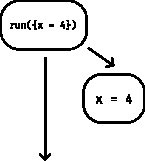
\includegraphics[alt={a flowchart showing a root node with the text run({x = 4}). It has two outgoing paths: a straight downward arrow pointing to the label UNKNOWN, and a diagonal downward-right arrow pointing to a state node with the text x = 4}]{exunknown} & 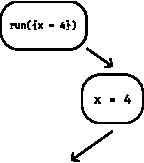
\includegraphics[alt={a flowchart showing a root node with the text run({x = 4}). It has a single outgoing path a diagonal downward-right arrow pointing to a state node with the text x = 4}]{exexactly_once} & 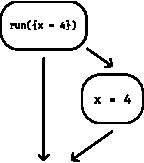
\includegraphics[alt={}]{exat_most_once} & 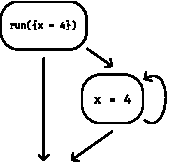
\includegraphics[alt={}]{exat_least_once} \\
%   \kt{UNKNOWN} & \kt{EXACTLY_ONCE} & \kt{AT_MOST_ONCE} & \kt{AT_LEAST_ONCE} \\
% \end{tabular}
% \caption{Sketch of the Kotlin CFG for lambda parameters in the presence of contracts.}
% \label{fig:cip-cfg}
% \end{figure}

Contracts exist for lambda parameters called \kt{EXACTLY\_ONCE}, \kt{AT\_LEAST\_ONCE} and \kt{AT\_MOST\_ONCE}, as well as a default \kt{UNKNOWN} value that falls back to the default behavior. In practice, the analysis phase implements these checks in two different passes, working together to compile the necessary information:
\begin{enumerate}
  \item a simple dataflow analysis on function bodies checks that they respect the contract declared in their signature;
  \item at call site, the CFG is rewritten (later showcased in Figure~\ref{fig:fduke-cfg}), adding edges based on the contract, and propagating the side effects of the lambda body to the local analysis.
\end{enumerate}
These rewrites increase the precision of the analysis by inlining the lambda body with edges that congruous with the function's contract. These new edges make intuitive sense with the language's semantics, but they are far from trivial: it's not clear on first glance why the result reached after considering them would be sound. Additionally, the rewrites rely on the correctness of the counting analysis, making the machinery around them brittle. Function contracts have been an experimental Kotlin feature since 2018, with their design being the subject of large amounts of scrutiny and discussion.

While type systems have systematic ways to study their interaction with semantics, these dataflow techniques, in the formulation they usually have in production compilers, have not enjoyed the same level of study. Our framework reduces this gap by obtaining proper, workable guarantees and by allowing for specifying these analyses and relating them back to program executions.

% Let us now present our framework.

% ===========================================================================
\section{Design and implementation}
\label{sec:design}

Before we can return to Kotlin and the analyses that we formalized, we describe the framework in Lean alongside the obligations that are put on the user. Once the language designer fulfills them, they obtain a theorem on the correctness of their analysis, a relation between the abstract state computed by the algorithm and the concrete state arising from execution. We call this relation \emph{coherence}, and denote it by $\coh \subseteq L \times S$, where $L$, $S$ are the abstract and concrete state spaces respectively. It serves as a stuttering simulation invariant between the abstract and the concrete. As we will see later, this coherence relation is chosen by the user depending on her goals, this allows full flexibility in the theorems one wants to prove, while maintaining the proof burden to a minimal amount.

Classical abstract interpretation methods would establish a connection between abstract and concrete states through a Galois connection: given spaces $L, S$, one would have to determine functions $\alpha : S \to L$, $\gamma : L \to S$ to obtain preorders on both, which encode precisely the information that the analysis should provide. While some presentations make this more suitable for formal methods work (like Pichardie's $\gamma$-only formulation~\cite{picha2005}), finding a good $\alpha, \gamma$ pair requires an uncomfortable amount of backwards thinking about the guarantees that one wishes to achieve, encoding a relation between two spaces $S$ and $L$ as a pair of two projections instead of phrasing it directly. $\coh$ works exactly as that direct relation, and the framework is built around making it easy for the user to work from this relation towards a full proof of correctness.

In the rest of this section we explain the most important components of the mechanized framework in Lean, while highlighting the obligations put on a user. We conclude it with a proof of Theorem~\ref{thm:framework}, certifying the soundness of an analysis.

\subsection{CFGs}

A CFG is represented as a list of abstract nodes, and a list of edges between them. We require an API to extract source and destination nodes from an edge (\lean{srcOf} and \lean{dstOf} respectively), as well as well-formedness conditions on both. We additionally distinguish a special \lean{entry} node to start the analysis from.

\begin{lstlisting}[language=Lean]
class AnalysisCFG (Node Edge : Type)
    [DecidableEq Node] [DecidableEq Edge] where
  nodes : List Node
  edges : List Edge
  entry : Node
  srcOf : Edge -> Node
  dstOf : Edge -> Node
  entry_mem : entry ∈ nodes
  srcOf_mem :
    ∀ e ∈ edges, srcOf e ∈ nodes
  dstOf_mem :
    ∀ e ∈ edges, dstOf e ∈ nodes
\end{lstlisting}

The well-formedness conditions could instead be enforced with the use of a dependent type \lean{NodeOf g} carrying its membership proof, but that proved to be more burdensome for the user, and the more explicit formulation was maintained. The \lean{Node} and \lean{Edge} types are deliberately abstract to allow full flexibility in the end user's choice of model.

\subsection{Finite height bounded semilattices}

The properties of finite-height, bounded semilattices lie at the core of monotone frameworks, and most of the properties we provide, like termination and soundness, follow directly from them. Analyses in our framework are stated over join-semilattices (isomorphic to their meet counterpart), so we describe them in detail.

We say that a type is of \emph{finite height} with the following typeclass:

\begin{lstlisting}[language=Lean]
class FiniteHeight (L : Type) [Max L] where
  remainingHeight : L -> Nat
  height_join : ∀ a b, a ⊔ b ≠ a -> remainingHeight (a ⊔ b) < remainingHeight a
\end{lstlisting}

We require every chain in $L$ to have a decreasing bounded measure, meaning that any join between two elements strictly decreases the measure of its operands, if it is not equal to them. The finite-heightness requirement on lattices is required to guarantee termination. While all of the analyses we consider are defined over lattices of finite height, other techniques to establish termination exist, such as widening; we will not consider them here as these are not used in Kotlin.

With this definition, we can define semilattices. Consider a join operation $\cdot \lub \cdot : L \times L \to L$ over elements of type $L$. This operation induces an ordering. For all $a, b \in L$, $a \squb b \;\equiv\; a \lub b = b$.

We say that a lattice is \emph{bounded} if there exists a distinguished element $\bot : L$ such that $\forall a \in L,\ \bot \squb a$.

With these definitions in hand, modelling the \textbf{F}inite \textbf{H}eight\\
\textbf{B}ounded \textbf{S}emi\textbf{lattice} (\fhbsl{}) is relatively straightforward:

\begin{lstlisting}[language=Lean]
class FHBSLattice (L : Type) [Max L] [Bot L] [FiniteHeight L] where
  join_comm  : ∀ a b : L, a ⊔ b = b ⊔ a
  join_assoc : ∀ a b c : L, (a ⊔ b) ⊔ c = a ⊔ (b ⊔ c)
  join_idem  : ∀ a : L, a ⊔ a = a
  bot_le     : ∀ a : L, ⊥ ⊑ a
\end{lstlisting}

\paragraph{Generic \fhbsl{}s.}
There are a few very common shapes of lattices that appear when designing analyses. We provide templates for those and prove that they too are \fhbsl:
\begin{itemize}
  \item \textbf{The product lattice}: given two \fhbsl{}s $L_1$ and $L_2$, $L_1 \times L_2$ is a \fhbsl{} with $(a_1, a_2) \lub (b_1, b_2) = (a_1 \lub_1 b_1,\ a_2 \lub_2 b_2)$.
  \item \textbf{The boolean lattice}: $\{\bot, \top\}$ is a lattice with
    $a \lub b = \begin{cases} \bot & \text{if } a = b = \bot \\ \top & \text{otherwise} \end{cases}$.
  \item \textbf{The domain lattice}: given a \fhbsl{} $L_1$ and $n \in \mathbb{N}$, the map $\Fin\, n \to L_1$ is a \fhbsl{} with $m_1 \lub m_2 = \lambda i.\ m_1(i) \lub_1 m_2(i)$. Here, $\Fin\, n$ represents a finite type of size exactly $n$.
  \item \textbf{The powerset lattice}: given an $n \in \mathbb{N}$, the powerset lattice is represented using the domain lattice with $n$ and the boolean lattice. This encodes the lattice of characteristic functions of a set. One can see that this induces the join to be set union and the order to be the subset relation.
\end{itemize}
In particular, the domain lattice is very useful, as it allows us to represent the finite number of variables in a program.

\subsection{Language semantics and dataflow analysis}

Our framework is only as useful as it allows us to relate abstract structures to real-world constructs. We do so by allowing the user to define their language semantics on the CFG they provide:

\begin{lstlisting}[language=Lean]
class LangSem (Edge Node State : Type) where
  LStep    : Edge -> State -> State -> Prop
  LStutter : Node -> State -> State -> Prop
  IsInit   : State -> Prop
\end{lstlisting}

The framework requires a stepping relation on the edges of the CFG, to relate input and output states. Since the abstract and concrete semantics might not always be completely synchronized, we allow the user to provide an \lean{LStutter} condition for a given node, to allow the concrete semantics to take a step that has no corresponding CFG transition. Finally, we ask of the user to define a predicate characterizing all possible initial states. On these semantics we define a reachability condition over states, as the reflexive transitive closure of \lean{LangSem.LStep} and \lean{LangSem.LStutter} starting from any state such that \lean{LangSem.IsInit}.

The desired properties of \lean{LangSem} are expressed in terms of a dataflow analysis (DFA). To specify an analysis it is enough to provide the transfer functions and the starting lattice value.

\begin{lstlisting}[language=Lean]
structure DFA (Node Edge : Type) where
  L : Type
  nodeTransfer : Node -> L -> L
  edgeTransfer : Edge -> L -> L
  entry : L
\end{lstlisting}

We additionally define \lean{transferAlong}, which composes the edge and node transfer functions, computing the in-state of the destination node from the in-state of a source node.

\begin{lstlisting}[language=Lean]
def DFA.transferAlong (A : DFA Node Edge) (e : EdgeOf g) (ℓ : A.L) : A.L :=
  A.edgeTransfer e (A.nodeTransfer (g.srcOf e) ℓ)
\end{lstlisting}

With this, we are ready to state the required properties of the dataflow analysis with regards to some language semantics.

\begin{lstlisting}[language=Lean]
structure DFASemantics (A : DFA Node Edge) where
  Coh : A.L -> State -> Prop
  preserve_entry :
    ∀ {σ : State}, LangSem.IsInit σ -> Coh A.entry σ
  preserve_step :
    ∀ {e : Edge} {σ σ' : State} {ℓ : A.L},
      LangSem.LStep e σ σ' -> Coh ℓ σ -> Coh (A.transferAlong g e ℓ) σ'
  preserve_stutter :
    ∀ {n : Node} {σ σ' : State} {ℓ : A.L},
      LangSem.LStutter g n σ σ' -> Coh ℓ σ -> Coh ℓ σ'
\end{lstlisting}

This is where the user finally defines their $\coh$ relation, and where they are required to show that:
\begin{enumerate}
  \item $\coh$ relates the abstract entry value to any initial concrete state;
  \item $\coh$ is preserved when a related abstract transfer application and concrete step along the CFG take place;
  \item $\coh$ is preserved when the concrete semantics take a step on a node on which the semantics stutter.
\end{enumerate}
These simple definitions are enough for users to define complex analyses, and establish non-trivial correctness relations for them. These obligations seem heavy, but they allow the framework to run the analysis algorithm and obtain guarantees on the result. Let us discuss what those guarantees are, and how they are established.

\subsection{Kildall's worklist algorithm}

To drive our analyses, we implement and verify the worklist algorithm on \fhbsl{}s as described in~\cite{Kildall73}. Provided a CFG $g = (N, E)$ and a DFA with transfer functions $f_n, f_e$, the algorithm runs to refine $\rho : N \to L$ into its post-fixpoint:
\[
  \forall n \in N,\ \forall s \in \succG_G(n),\quad f_n(\rho(n)) \squb \rho(s)
\]
The algorithm works by maintaining a worklist $l$ of nodes to process. We initialize $\rho$ to $\rho_0$, mapping every node into $\bot$, and $l$ to $N$.

Let $(\rho, l) \rightsquigarrow (\rho', l')$ denote a single step (an iteration) of the algorithm. When processing a node $n \in l$, $\rho'$ is computed by joining the results of the $f_{(n', n)}$ on all of its incoming edges, before applying the corresponding $f_n$ and joining it with the current state $\rho(n)$. Mathematically, this yields:
\[
  \rho'(n) = \rho(n) \lub f_n\Bigl(\bigsqcup_{n' \in \pred_G(n)} f_{(n', n)}\bigl(\rho(n')\bigr)\Bigr)
\]
If $\rho'(n)$ is different from $\rho(n)$, we append the successors of $n$ to the worklist, since they were affected by the change. This process continues until the worklist is empty. This procedure might be simple, but it is enough to compute a post-fixpoint solution, and to guarantee termination on finite height domains. We sketch the proofs of those properties here:

\begin{theorem}
The worklist algorithm terminates.
\end{theorem}

\begin{proof}
We argue that the measure $(h, l) \in \mathbb{N} \times \mathbb{N}$ decreases with every iteration, where $h$ is the sum of the remaining height of $\rho(n)$ for every $n \in N$, and $l$ is the length of the worklist. Let $\rho(n), \rho'(n)$ be the abstract values at $n$ before and after an iteration. Since $a \squb a \lub b$, we know that $\rho(n) \squb \rho'(n)$. We therefore have two cases: if $\rho(n) = \rho'(n)$ there was no change, so $l$ decreases. Otherwise, a better result was found, so $h$ decreases. \qed
\end{proof}

This argument only holds because of the finite height of our lattice, which gives us a lower bound we can decrease towards. To show that the result of this algorithm is a post-fixpoint, we borrow a technique from~\cite{LaSpina25} to establish invariants over the algorithm's runtime.

We say that a property $P$ over an intermediate analysis result $\rho$ and a worklist $l$ is \emph{inductive} if $P(\rho_0, l_0)$ and $P(\rho, l) \to \bigl((\rho, l) \rightsquigarrow (\rho', l')\bigr) \to P(\rho', l')$ where $\rightsquigarrow$ denotes a single iteration of the algorithm as before. We denote the final result of the algorithm with $\overline{\rho}$. Then, we can show the following intermediate result:

\begin{lemma}\label{thm:iteration-inv}
Let $P$ be an inductive property. Then, $P(\overline{\rho}, [\,])$.
\end{lemma}

\begin{proof}
By induction on the iterations of the algorithm. \qed
\end{proof}

Using this result, the proof of soundness is relatively straightforward.

\begin{theorem}\label{thm:soundness}
For any $n \in N$, and any transfer function $f_n$, the result of the worklist algorithm $\overline{\rho}$ is a post-fixpoint.
\end{theorem}

\begin{proof}
It is easy to check that $P(\rho, l) = $ ``$\rho$ is a post-fixpoint for all $n \notin l$'' is inductive. We apply Lemma~\ref{thm:iteration-inv} with $P$, concluding the proof. \qed
\end{proof}

% Interestingly, this soundness result does not require the transfer functions in the analysis to be monotonic. Monotonic transfer functions allow us to show that $\overline{\rho}$ is a \emph{least} post-fixpoint, a result that is mechanized in our framework but that goes unused in our case studies.
% Using Theorem~\ref{thm:soundness}, we can finally state and prove the main theorem of the framework, Theorem~\ref{thm:framework}.

With this result, we can finally prove our final theorem: 
\begin{theorem}\label{thm:framework}
Let $g = (N, E)$ be a CFG with semantics relating states in $S$. Given an analysis $A$ with transfer functions over a bounded semilattice $L$, and a relation $\coh \subseteq L \times S$ that is preserved under semantics steps, the post-fixpoint $\rho : N \to L$ of the transfer functions from $A$ on $g$ is such that for all reachable states $\sigma : S$ at node $n \in N$, $\coh(\rho(n), \sigma)$ holds.
\end{theorem}

\begin{proof}
By induction on the steps, using \lean{DFASemantics} initialization and preservation properties, together with the soundness of the Kildall algorithm from Theorem~\ref{thm:soundness}. \qed
\end{proof}

With the guarantees established, we move onto discussing our application of the framework, showing its full power in action.

% ===========================================================================
\section{Application}
\label{sec:appl}

We implement our analyses on Duke, an untyped imperative language designed to be a simple subset of Kotlin. It contains the required language constructs for the nullability analysis.

Values $\Val$ are represented by potentially nullable integers. Values which are either null or the integer 0 are considered falsy. Strictly positive integers are considered truthy. Statements consist of variable declarations, assignments, if- and while-statements; the syntax is defined in Figure~\ref{fig:duke-syn}. By allowing values to be nullable, we model Kotlin's approach to flow typing, including the use of \emph{consequents} which we will present shortly.

\begin{figure}[t]
\centering
\begin{align*}
  \oplus & \Coloneqq {+} \mid {-} \mid {*} \mid {<} \mid {=} \mid {\wedge} \\
  e      & \Coloneqq \knull \mid \kInt\ n \mid \kVar\ x \mid \kisnull\ e \mid {!}\,e \mid e \oplus e \\
  s      & \Coloneqq \kvar\ x \coloneqq e \mid x = e \mid \kif \, (e) \, \{s\} \, \kelse \, \{s\} \\
         & \quad\;\; \mid \kwhile \, (e) \, \{s\} \mid \kskip \mid s\,;\,s
\end{align*}
\caption{Syntax of Duke}
\label{fig:duke-syn}
\end{figure}

To define the concrete semantics of Duke, we must first present its CFG construction. We represent nodes with simple identifiers $\NodeID$, where edges are pairs of such $\NodeID$s. We use $\NodeKind$ to differentiate program constructs:
\[
  \NodeKind \Coloneqq x = e \mid \kassume\ e \mid \kskip
\]
The assignment node simply binds the value of the expression $e$ to the variable named $x$. The synthetic assume node is inserted after conditionals, to indicate which branch was taken, and the abstract interpreter will assume that its condition holds, mimicking Kotlin's CFG. Finally, $\kskip$, is a node with no action attached to it.

\begin{figure}[t]
\centering
\begin{tabular}{cccc}
  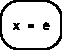
\includegraphics[alt={a single control flow graph node containing the text x = e}]{decl} &
  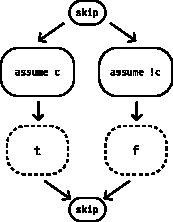
\includegraphics[alt={a control flow graph with a top skip node branching into two paths: a left branch pointing to assume c leading to the embedded node t, and a right branch pointing to assume !c leading to the embedded node f. Both t and f nodes merge down into a bottom skip node}]{if} &
  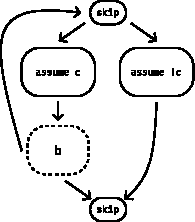
\includegraphics[alt={a control flow graph with a top skip node that branches into two paths: a left branch pointing to assume c leading to the embedded node b, which loops back to the top skip node; and a right branch pointing to assume !c which bypasses the loop and leads directly down to a bottom skip node.}]{while} &
  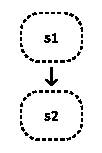
\includegraphics[alt={a control flow graph of the embedded s1 node connected to the embedded s2 node}]{seq} \\
  $\kvar\ x \coloneqq e,\ x = e$ & $\kif \, (c) \, \{t\} \, \{f\}$ & $\kwhile \, (c) \, \{b\}$ & $s_1 ; s_2$ \\
\end{tabular}
\caption{Statement to CFG translation for Duke. Dotted nodes represent subgraphs.}
\label{fig:duke-cfg}
\end{figure}

In Figure~\ref{fig:duke-cfg} we show the translation of Duke's statements into its CFG. A conditional over an expression $c$ always create two edges from a skip node into nodes for $\kassume\ c$ and $\kassume\ {!}c$. We define a big-step reduction for expressions into values, for which select rules are available in Figure~\ref{fig:expr-eval}, where $\sem{\oplus}$ denotes the interpretation of the binary operator $\oplus$. We represent the environment map with $\sigma : \Var \harpoon \Val$. Notice that we can have stuck terms in three cases:
\begin{enumerate}
  \item if either operand of $\oplus$ is null, or
  \item if the operand of $!$ is null, or
  \item if for $\kVar\ x$, $x$ is not defined in $\sigma$.
\end{enumerate}

With that, we define the concrete semantics on the CFG, in Figure~\ref{fig:cfg-sem}, as reductions on $(n, \sigma) \in N \times (\Var \harpoon \Val)$.
% They are designed to integrate pretty naturally with the existing features of the \Chartreux{} framework, all while remaining the fundamental ground-truth semantics for this language.

We again encounter reductions which can get stuck, either because an expression reduction failed or because an assume node contains a falsy expression. It will be precisely the role of the dataflow analysis to show that properly formed programs cannot get stuck during execution.

When integrating all of the above with \Chartreux, we can think about what steps are loud and which are stutter: since CFG reductions are the ground truth \lean{LStep} semantics, we do not have to define anything as stutter as there is no correspondence to be drawn. The concrete state \lean{State} simply becomes $\Var \harpoon \Val$.

\begin{figure}[t]
\centering
\begin{mathpar}
  \inferrule*[right=Null]{ }{\sigma \vdash \knull \Downarrow \knull}
  \and
  % \inferrule*[right=Int]{ }{\sigma \vdash \kInt\ n \Downarrow \kInt\ n}
  % \and
  % \inferrule*[right=Var]{\sigma(x) = v}{\sigma \vdash \kVar\ x \Downarrow v}
  % \\
  \inferrule*[right=IsNull-T]{\sigma \vdash e \Downarrow \knull}{\sigma \vdash \kisnull\ e \Downarrow \kInt\ 1}
  \and
  \inferrule*[right=IsNull-F]{\sigma \vdash e \Downarrow v \\ v \ne \knull}{\sigma \vdash \kisnull\ e \Downarrow \kInt\ 0}
  \and
  % \inferrule*[right=Not-T]{\sigma \vdash e \Downarrow \kInt\ n \\ n \ne 0}{\sigma \vdash {!}\,e \Downarrow \kInt\ 0}
  % \and
  % \inferrule*[right=Not-F]{\sigma \vdash e \Downarrow \kInt\ 0}{\sigma \vdash {!}\,e \Downarrow \kInt\ 1}
  % \\
  \inferrule*[right=BinOp]{\sigma \vdash e_1 \Downarrow \kInt\ n_1 \\ \sigma \vdash e_2 \Downarrow \kInt\ n_2 \\ v = n_1 \sem{\oplus} n_2}
    {\sigma \vdash e_1 \oplus e_2 \Downarrow v}
\end{mathpar}
\caption{Big-step semantics for Duke $\knull$ values.}
\label{fig:expr-eval}
\end{figure}

\begin{figure}[t]
\centering
\begin{mathpar}
  \inferrule*[right=Assign]{\kind(n) = (x = e) \\ \sigma \vdash e \Downarrow v \\ n' \in \succG(n)}
    {(n, \sigma) \to (n', \sigma[x \mapsto v])}
  \and
  \inferrule*[right=Assume]{\kind(n) = \kassume\ e \\ \sigma \vdash e \Downarrow \kInt\ m \\ m \ne 0 \\ n' \in \succG(n)}
    {(n, \sigma) \to (n', \sigma)}
  \and
  \inferrule*[right=Skip]{\kind(n) = \kskip \\ n' \in \succG(n)}
    {(n, \sigma) \to (n', \sigma)}
\end{mathpar}
\caption{Duke CFG Semantics. $\kind : \NodeID \to \NodeKind$ identifies node IDs with their kinds.}
\label{fig:cfg-sem}
\end{figure}

\subsection{Nullability with consequents}

The point of nullability analysis is to statically determine which values might be null at every point in the program, to avoid invalid dereferences. We present a nullability analysis with \textit{boolean witnesses}, which we show guarantees the absence of stuck terms.

We first need a few lattices. First, $\AbsVal$:
\begin{center}
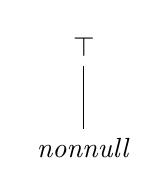
\begin{tikzpicture}[node distance=0.8cm]
  \node (top) {$\top$};
  \node (bot) [below=of top] {$\nonnull$};
  \draw (bot) -- (top);
\end{tikzpicture}
\end{center}
which determines whether a value is definitely $\nonnull$ or unclear ($\top$), and is clearly finite-height. This is of finite height since it has a finite amount of elements. The join is defined as follows:
% might not be needed
\begin{align*}
  \nonnull \lub a = a \lub \nonnull & \coloneqq a \\
  \top \lub \top & \coloneqq \top
\end{align*}
% might not be needed
The bottom element of $\AbsVal$ is $\nonnull$. The join (and the induced order) fulfills the requirements of being a \fhbsl.

Next, we use the domain lattice template to create $\AbsConseq : \Var^n \to \AbsVal$, which is also a \fhbsl,   since $\AbsVal$ is. It stores the consequent of the implication that if a variable is truthy, then the assertions in $\AbsConseq$ hold. For example, in the program $x = {!}(\kisnull\ y) \wedge {!}(\kisnull\ z)$, not only do we know that $x$ is $\nonnull$, but also that it is a witness of $y$ and $z$ being $\nonnull$. If $x$ evaluates to a truthy value, we will know both $y$ and $z$ is not null. This makes our domain relational.
% what is a relational domain?

Finally, since we want to store nullability information for each variable separately, we wrap $\AbsVal$ and $\AbsConseq$ in a domain over all variables, $\AbsFact : \Var^n \to \AbsVal \times \AbsConseq$. Since both $\AbsVal$ and $\AbsConseq$ are \fhbsl{}s, so is $\AbsVal \times \AbsConseq$, and for the same reason, $\AbsFact$.
% Similarly, so is the entire $\AbsFact$.

% really needed?
To illustrate this lattice, consider these $\AbsFact$ instances, representing the program points in Figure~\ref{lst:nullability-example}:
\begin{enumerate}
  \item $\mathit{cost} \mapsto (\nonnull, \{\mathit{cost} \mapsto \top, \mathit{valid} \mapsto \top\})$\\
        $\mathit{valid} \mapsto (\top, \{\mathit{cost} \mapsto \top, \mathit{valid} \mapsto \top\})$
  \item $\mathit{cost} \mapsto (\top, \{\mathit{cost} \mapsto \top, \mathit{valid} \mapsto \top\})$\\
        $\mathit{valid} \mapsto (\nonnull, \{\mathit{cost} \mapsto \nonnull, \mathit{valid} \mapsto \top\})$
  \item $\mathit{cost} \mapsto (\nonnull, \{\mathit{cost} \mapsto \top, \mathit{valid} \mapsto \top\})$\\
        $\mathit{valid} \mapsto (\nonnull, \{\mathit{cost} \mapsto \nonnull, \mathit{valid} \mapsto \top\})$
\end{enumerate}
To define the transfer functions, we first need to define abstract evaluation of expressions:
\begin{align*}
  \aeval : \AbsFact \times \Expr & \to \AbsVal \\
  \aeval(\rho, \knull)        & \coloneqq \top \\
  \aeval(\rho, \kInt\ n)      & \coloneqq \nonnull \\
  \aeval(\rho, \kVar\ x)      & \coloneqq \fst(\rho(x)) \\
  \aeval(\rho, \kisnull\ e)   & \coloneqq \nonnull \\
  \aeval(\rho, {!}\,e)        & \coloneqq \nonnull \\
  \aeval(\rho, e_1 \oplus e_2) & \coloneqq \aeval(\rho, e_1) \lub \aeval(\rho, e_2)
\end{align*}
We also need a way to use obtain consequents from a given expression, which means answering the question ``given an expression $e$, what nullability information do we gain when assuming $e$ is truthy?''.
\begin{align*}
  \exprConseq : \AbsFact \times \Expr & \to \AbsConseq \\
  \exprConseq(\rho, \kVar\ x) & \coloneqq \lambda y.
    \begin{cases} \nonnull & \snd(\rho(x))(y) = \nonnull \\ \top & \text{otherwise} \end{cases} \\
  \exprConseq(\rho, {!}\,\kisnull\ (\kVar\ x)) & \coloneqq \lambda y.
    \begin{cases} \nonnull & x = y \\ \top & \text{otherwise} \end{cases} \\
\exprConseq(\rho, e_1 \wedge e_2) & \coloneqq \lambda y.
    \begin{cases}
      \nonnull & \exprConseq(\rho, e_1)(y) = \nonnull \;\vee \\
               & \quad \exprConseq(\rho, e_2)(y) = \nonnull \\
      \top     & \text{otherwise}
    \end{cases} \\
  \exprConseq(\rho, e) & \coloneqq \lambda \_.\ \top
\end{align*}
When looking at a variable we consult the consequents that variable holds. If we assume ${!}\,\kisnull\ (\kVar\ x)$ holds, it of course means that $x$ is not null. In case of a conjunction we consider both sides holding true. Finally, for all other cases there is nothing we can say.

This allows us to define the node transfer function:
\begin{align*}
  f : \NodeKind \to \AbsFact & \to \AbsFact \\
  f(x = e)(\rho) & \coloneqq \lambda y.
    \begin{cases}
      (\aeval(\rho, e),\ \exprConseq(\rho, e)) & x = y \\
      (\fst(\rho(y)),\ \lambda \_.\ \top) & \text{otherwise}
    \end{cases} \\
  f(\kassume\ e)(\rho) & \coloneqq \lambda y.
    \begin{cases}
      (\nonnull,\ \snd(\rho(y))) & \exprConseq(\rho, e)(y) = \nonnull \\
      \rho(y) & \text{otherwise}
    \end{cases} \\
  f(\kskip)(\rho) & \coloneqq \rho
\end{align*}
Where $\fst$ and $\snd$ are standard projection functions to the first and second element respectively. In the case of assignment $x = e$, we assign the $\AbsVal$ to $x$ from the abstract evaluation of $e$ and we extract the consequents coming from $e$. For all other variables in the program we keep their $\AbsVal$, but invalidate all consequents, since the mutation might have invalidated them. The transition for $\kassume\ e$ extracts the consequents from $e$ and immediately assumes them to hold.

\subsubsection{Correctness.}
For an abstract state $\rho : \AbsFact$ and a concrete state $\sigma : \mathit{State}$, we define the following coherence relation:
\begin{align*}
  \coh(\rho, \sigma) = {} & \forall x \in \dom(\rho). & \\
  & \bigl[\fst(\rho(x)) = \nonnull \to \sigma(x) \neq \knull\bigr] \wedge {} & (1)\\
  & \bigl[\forall y \in \dom(\rho).\ \snd(\rho(x))(y) = \nonnull \; \wedge & (2)\\
  & \; \; \; \; \sigma(x) = \kInt\ n \wedge n \neq 0 \to \sigma(y) \neq \knull\bigr] &
\end{align*}
Where $(1)$ is the analysis' correctness property, and $(2)$ is the denotation for consequents, needed for the proof of step preservation. Once all proofs are completed, we can combine this analysis with a standard initialization analysis, leading to Duke's safety theorem:

\begin{theorem}
Let $g$ be a program such that successful initialization and nullability analyses have been carried out. Let $(n, \sigma)$ be a reachable execution configuration when running $g$. Then, either:
\begin{itemize}
  \item $n$ is the exit node of $g$;
  \item $n$ is an $\kassume$ node whose condition is false;
  \item there exists a node $n'$ and a state $\sigma'$ such that $(n, \sigma) \to (n', \sigma')$.
\end{itemize}
\end{theorem}

At exit nodes we naturally cannot take a step, and since an $\kassume\ c$ node is always paired with $\kassume\ {!}c$, one of them must be necessarily false.

\subsection{Function contract checking}

The second problem concerns the CFG rewrites induced by calls-in-place contracts. A call node is followed by a copy of the body of the lambda, with surrounding edges marking whether the lambda may be skipped or repeated. This allows the caller's analysis to gather more information, but it introduces a new burden in verifying that these rewrites are indeed correct.

We study this problem in \emph{FDuke}, an extension of Duke with function calls and lambda invocation. Its statements have two additional forms:
\[
  s \Coloneqq \ldots \mid \kcall\ f\ \{s\} \mid \kinvoke
\]
The statement $\kcall\ f\ \{s\}$ passes $s$ as the closure argument of $f$, while $\kinvoke$ executes the current function's closure argument. Lambdas have no parameters of their own, but execute in the store captured at the call site. A program consists of a main statement and a finite function environment $\Phi : \Id \harpoon (\kappa \times \Stmt)$. The invocation kind $\kappa \in \{\varepsilon, 1, +, ?\}$ denotes, respectively, an unknown number of invocations, exactly one, at least one, or at most one.

\begin{figure}[t]
\centering
\begin{tabular}{cccc}
  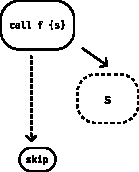
\includegraphics[alt={a control flow graph with a top node call f {s} pointing both to an embedded s node and with a dotted arrow to a bottom skip node}]{unknown} & 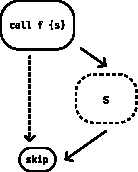
\includegraphics[alt={a control flow graph with a top node call f {s} pointing both to an embedded s node and with a dotted arrow to a bottom skip node; additionally the embedded s node is connected to the bottom skip node}]{exactly_once} & 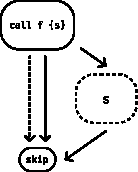
\includegraphics[alt={a control flow graph with a top node call f {s} pointing both to an embedded s node and with both a dotted and solid arrow to a bottom skip node; additionally the embedded s node is connected to the bottom skip node}]{at_most_once} & 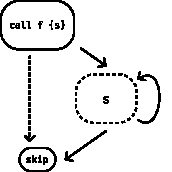
\includegraphics[alt={a control flow graph with a top node call f {s} pointing both to an embedded s node (which has a self loop) and with a dotted arrow to a bottom skip node; additionally the embedded s node is connected to the bottom skip node}]{at_least_once} \\
  $\varepsilon$ & $1$ & $?$ & $+$ \\
\end{tabular}
\caption{Contract-dependent CFG fragments in FDuke. The lambda body $\{s\}$ is copied into the caller for analysis; the dotted arrow depicts the CEK machine's call/return control transfer and is not an edge of the analysis graph.}
\label{fig:fduke-cfg}
\end{figure}

For a call node with lambda entry $\mathrm{en}_L$, lambda exit $\mathrm{ex}_L$, and return node $r$, the lowering emits the fragments in Figure~\ref{fig:fduke-cfg}. The resulting paths execute the inlined body any number of times admitted by the contract:
\begin{align*}
  \admits(\varepsilon, k) & \coloneqq \top \\
  \admits(1, k) & \coloneqq (k = 1) \\
  \admits(+, k) & \coloneqq (1 \leq k) \\
  \admits(?, k) & \coloneqq (k \leq 1).
\end{align*}
The lowering also records some metadata for the callsite: the call node, callee, lambda identifier, invocation kind, inline entry and exit, return node, and source lambda body. The dotted arrow in Figure~\ref{fig:fduke-cfg} represents how the concrete CEK machine uses this metadata to enter the callee and eventually return to $r$.

\subsubsection{Concrete semantics.}
Lowering an FDuke program produces a family of CFGs: one graph for \kt{main}, one for each function body, and one for every lambda literal. The semantics relate configurations of the form $\langle n, \sigma, \rho, K \rangle$, where $n$ identifies both a graph and a node, $\sigma$ is the current store, $\rho$ is an optional closure, and $K$ is a stack of continuations. A closure records a lambda's entry and exit nodes, its captured closure, and its captured store.

\begin{figure}[t]
\centering
\begin{mathpar}
  \inferrule*[right=Call]
    {\kind(n) = \kcall\ f\ \{\ell\} \\ r \in \succG_{\summary}(n)}
    {\langle n, \sigma, \rho, K \rangle \to
     \langle \mathrm{en}_f, \cdot, \some(C), \kcall r \{\rho\} :: K \rangle}
  \and
  \inferrule*[right=Invoke]
    {\kind(n) = \kinvoke \\ \rho = \some(\langle\mathrm{en}_L, \mathrm{ex}_L, \rho_d, \sigma_d\rangle) \\ r \in \succG(n)}
    {\langle n, \sigma, \rho, K \rangle \to
     \langle \mathrm{en}_L, \sigma_d, \rho_d, \mathrm{inv}(r, \rho, \sigma) :: K \rangle}
  \and
  \inferrule*[right=Return-Call]
    {\succG(n) = \emptyset}
    {\langle n, \sigma, \some(\langle \mathrm{en}_L, \mathrm{ex}_L, \rho_c, \sigma_c\rangle), \kcall \, r \{\rho'\} :: K \rangle \to
     \langle r, \sigma_c, \rho_c, K \rangle}
  \and
  \inferrule*[right=Return-Invoke]
    {\succG(n) = \emptyset}
    {\langle n, \sigma, \rho', \mathrm{inv}(r, \some(\langle \mathrm{en}_L, \mathrm{ex}_L, \rho_d, \sigma_d \rangle), \sigma_f) :: K \rangle \to
     \langle r, \sigma_f, \some(\langle \mathrm{en}_L, \mathrm{ex}_L, \rho', \sigma \rangle), K \rangle}
\end{mathpar}
\caption{Function and invocation semantics}
\label{fig:function-semantics}
\end{figure}

The relevant rules are shown in Figure~\ref{fig:function-semantics}. Calling $f$ saves the lambda and the caller's store in a closure, starts the function body with an empty store, and pushes the return point. An $\kinvoke$ starts the saved lambda in its captured store and pushes the function's current store. Returning from the lambda updates the closure with the lambda's resulting store and resumes the function; returning from the function restores this store in the caller.

\subsubsection{Checking contracts.}
Before relying on a contract, we verify it with a counting analysis. Its domain is $\Cnt = \mathcal{P}(\{0, 1, \omega\})$, where $\omega$ represents two or more invocations. It is a finite-height powerset lattice ordered by inclusion, with union as join and the empty set as $\bot$. The entry value is $\{0\}$. At an $\kinvoke$ node, every possible count is incremented according to $0 + 1 = 1$, $1 + 1 = \omega$, and $\omega + 1 = \omega$; all other transfer functions are the identity.

The concrete semantics used for this analysis pairs the store with a ghost natural-number counter. Its coherence relation states that the abstraction of the concrete counter belongs to the current element of $\Cnt$. Incrementing the counter and applying the transfer function preserve coherence, so Theorem~\ref{thm:framework} establishes that every concrete invocation count reaching a node is included in the computed result.

Let $\overline{\rho}_f$ be a post-fixpoint obtained for the body of $f$, and let $n_f$ be its exit node. For a family $p$, we write $\FamilyChecked(p)$ when, for all $f$ in $p$, we have:
\begin{align*}
  1 & \leftrightarrow \overline{\rho}_f(n_f) = \{1\} \\
  + & \leftrightarrow 0 \notin \overline{\rho}_f(n_f) \\
  ? & \leftrightarrow \omega \notin \overline{\rho}_f(n_f).
\end{align*}

\subsubsection{Correctness of the rewrite.}
We relate the interprocedural CEK semantics to the analysis graph $\Gk$, by recognizing that we can represent a function call's effect by traversing its lambda body $k$ times, where $k$ is allowed by its contract fragment.

This direct account depends on certified lowering. For every call, the builder records a \emph{call gadget} containing the call and return nodes, inline-body endpoints, lambda identifier, invocation kind, and source body. It proves that all edges prescribed by that invocation kind are present. A certificate-bearing family additionally connects the inline copy to the separately generated lambda component, including the node offset, shifted lambda identifiers, edges, and nested call gadgets. Erasing the proofs recovers the execution-facing CFG family and preserves both component and gadget lookup. Consequently the projection never infers provenance from an arbitrary graph after the fact.

\begin{theorem}\label{thm:fduke-projection}
Let $p$ be an FDuke program such that $\FamilyChecked(p)$. Every CEK execution that starts and ends in the same CFG, in an empty continuation and with no closure, can be represented by a sequence of steps in its $\Gk$, with the same initial and final stores.
\end{theorem}

\begin{proof}[Sketch]
To prove this theorem, we consider the more general class of \emph{balanced} CEK runs, i.e. those whose continuation extends a fixed stack, and returns to exactly that stack. By strong induction on the length of these runs, we can show that there is always an equivalent run in $\Gk$: all "regular" steps match directly, and all runs of $\kinvoke$ or $\kcall$ are strictly shorter than the one we are currently considering, so the existence of a $\Gk$ run follows by induction, and our assumption that $\FamilyChecked(p)$ gives us that the rewrites are correct.

Specializing this lemma to the balanced run that starts and ends with an empty continuation gives us a proof of \ref{thm:fduke-projection}. \qed
\end{proof}

Now that we have a direct reachability correspondence between the interprocedural semantics and the $\Gk$ runs, we can apply Theorem~\ref{thm:framework}, to obtain our final result: every correct analysis remains correct in the presence of function calls:

\begin{theorem}\label{thm:fduke}
Let $p$ be an FDuke program with a checked function family, and let $g$ be one of its CFG components. Suppose an analysis $A$ over $\Gk$ has a coherence relation preserved by its transfer functions, and let $\rho$ be a post-fixpoint whose entry contains the analysis entry value. For every state $\sigma$ reached at node $n$ by a balanced CEK execution of $p$ from the entry of $g$, $\coh(\rho(n), \sigma)$ holds.
\end{theorem}

% ===========================================================================
\section{Discussion}
\label{sec:discuss}

\subsection{Future work}

This tool is under very active development. The end-to-end function-contract derivation presented here is mechanized, while \Chartreux{} as a framework has multiple paths for improvement. The integration of a WTO-based solver~\cite{LaSpina25} could provide better efficiency and accuracy of computed fixpoints. Additionally, it would be beneficial if the framework provided primitives for the handling of function calls, given the current burden on the users. Lastly, the framework could provide alternative formalization paths like allowing for non-finite height lattices with a widening operator, or letting the user define correctness by means of a Galois connection whenever more convenient.

On the other hand, a more complete formalization of Kotlin's analyses requires extending the verified function contract model with more realistic language constructs. In a real-world compiler, aliasing, exceptions, and other runtime dangers are real sources of hidden unsoundness, and our framework can be very useful in the study of such pitfalls. Additionally, formalizing part of Kotlin, and showing correspondence between regular small-step semantics and the CFG execution will increase our confidence that the CFG semantics are fully representative.

\subsection{Conclusion}
\label{sec:conc}

We describe the design and implementation of a foundational, language-agnostic, formally verified framework for exploration, specification, and verification of dataflow analyses that \emph{properly capture the semantics of the enclosed language}. The framework is minimal and low obligation. We apply it to modern analyses to obtain formal guarantees and increased understanding of the Kotlin language. We trace a clear path of future work to graduate this project from a proof of concept to a versatile, extensible and easy-to-use tool, as a companion to aid the tasks of analysis engineers.

\begin{credits}
\subsubsection{\ackname} We deeply thank Kameliya Golova for her mentoring throughout this work and for providing invaluable feedback on the paper.

\subsubsection{\discintname}
The authors have no competing interests to declare that are relevant to the content of this article.

\subsubsection{Data-Availability}
Chartreux, Duke/FDuke, and the analyses, are available at \url{https://github.com/korrektness/chartreux}.
\end{credits}


% ===========================================================================
\bibliographystyle{splncs04}
\bibliography{refs}   % keys: Cousots, Kotlin, kotlin-smart-casts, racket-occurrence-typing,
                      %       typescript-narrowing, Verasco, CompCert, iTree, picha2005,
                      %       Kildall73, LaSpina25

\end{document}